\chapter{Implementation}
\section{Hardware}
\begin{wrapfigure}{r}{0.24\textwidth}
    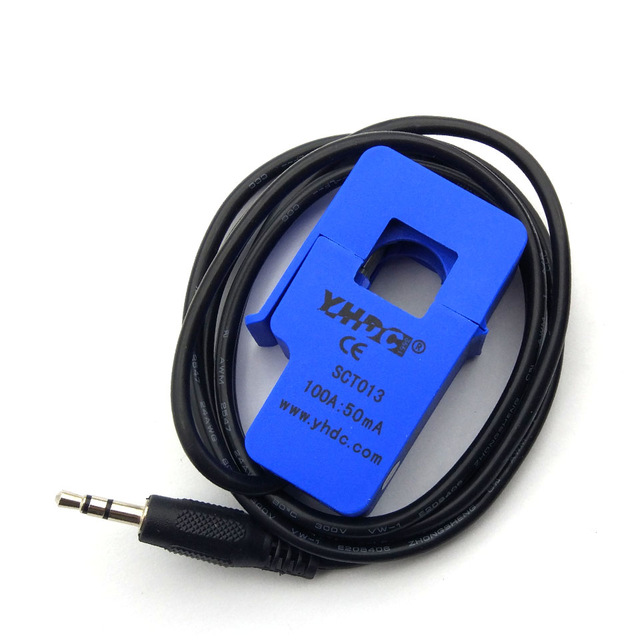
\includegraphics[width=0.9\linewidth]{YHDC-SCT013.jpg}
    \caption{\protect\raggedright YHDC-SCT013}
    %\vspace{-30pt}
    \label{fig:yhdc}
\end{wrapfigure}
As discussed in the introduction, there are multiple ways to collect data. For this project, we wanted a cheap solution easily usable for anyone wanting to use the project; making it more affordable for both users and contributors. This is why we use a generic split-core current transformer, like the one on \autoref{fig:yhdc}. It is simply wired into the sound card of any computer. This allows getting a sampling of more than 40kHz on most sound cards. However, we are going to sample at only around  4kHz since it seems to be as efficient for our current algorithm.

During the development of the project a laptop was used but since the CPU usage is very low, a single board computer running Linux (like a Raspberry Pi) should be more than enough to do the job, provided that it has an input on which you can plug the split core current transformer.


\section{Architecture}
The project is made to be modular. It is divided into multiple modules aiming at one particular task at a time. The identified tasks are as follow: gather the data, detect when there is a change in the data (i.e. the state of an appliance has changed) and finally detect what appliance it is. The process is described on \autoref{fig:process_diagram}. Everything is made so that the disaggregation can be made with different types of input data. In this case, we only use a current meter, but the only thing we need to redefine if we change the input data (like adding readings from a voltmeter and using the V-I trajectory -- see \autoref{section-vi}) would be to change the distance between two datapoints.

{\color{red}define signal} %TODO

In order to detect when changes in the signal occur, we need to have a base signal. This base signal is the one we should continuously have while there is no change on the network. Because there is a lot of noise due to small variations in the EMI -- due to changes in power needs -- , readings errors, and changes in the frequency of the electricity provider -- due to the imbalance of the production and the consumption --, we continuously need to smoothen the base signal. This smoothing occurs only if the read signal is not too far from the base signal, which is decided by \texttt{EventDetector}. If it is too far, then the few next readings are taken together and the mean is computed. The difference between this mean and the base signal is expected to be the signal emitted by the new appliance. If that appliance has already been registered, a copy of the data will automatically be added in the record of the appliance; if not a new appliance will be registered containing the new signal.


\tikzset{
    mynode/.style={rectangle,rounded corners,draw=black,very thick, inner sep=0.5em, minimum size=3em, text centered},
    method/.style={ellipse,draw=black,very thick, inner sep=0.01em, minimum size=3em, text centered},
    myarrow/.style={-triangle 45, >=latex', shorten >=1pt, very thick},
    mylabel/.style={text width=7em, text centered} 
} 

\begin{figure}
    \centering
    \begin{tikzpicture}[node distance=2cm, auto]  
    \node[mynode, fill=blue!30] (new_data) {New data};
    \node[mynode, left=1cm of new_data,draw=white] (start) {Start};
    \node[mynode, above right=1cm of new_data] (smoothen_base) {Smoothen Base};
    \node[mynode, below right=1cm of new_data] (smoothen_signal) {Smoothen Signal};
    \node[mynode, below left=of smoothen_signal] (add_data) {Add data to appliance};
    \node[mynode, below right=of smoothen_signal] (new_appliance) {Create new appliance};
    \node[mynode, below = 3cm of smoothen_signal] (signal) {Signal AND New base};
    \node[method, below = 0.5cm of smoothen_signal] (closest) {Get closest};
    \node[method, right = 0.5cm of new_data] (detect) {Detect ?};
    
    \draw[myarrow] (new_data) -- node [text width=2.5cm,below,align=center,sloped] {no} (smoothen_base);
    \draw[myarrow] (new_data) -- node [text width=2.5cm,above,align=center,sloped] {yes} (smoothen_signal);
    \draw[myarrow] (smoothen_signal) -- node [text width=2.5cm,below,align=center,sloped] {Distance below threshold} (add_data);
    \draw[myarrow] (smoothen_signal) -- node [text width=2.5cm,below,align=center,sloped] {Distance above threshold} (new_appliance);
    \draw[myarrow] (add_data) -- (signal);
    \draw[myarrow] (new_appliance) -- (signal);
    \draw[myarrow,dashed] (smoothen_signal) to [out=0,in=50,loop,looseness=4] node [text width=2.5cm,above,align=center,sloped]{Repeat}(smoothen_signal);
    \draw[myarrow] (signal.west) -- ++(-5.6,0) -- ++(0,4) -| (new_data);
    \draw[myarrow] (smoothen_signal.east) -- ++(1.5,0) -- ++(0,5) -| (new_data);
    \draw[myarrow] (smoothen_base.west) -- ++(-1,0) -| (new_data);
    \draw[myarrow] (start) -- (new_data);
    \end{tikzpicture}
    \caption{Process Diagram}
    \label{fig:process_diagram}
\end{figure}

\begin{figure}
    \centering
    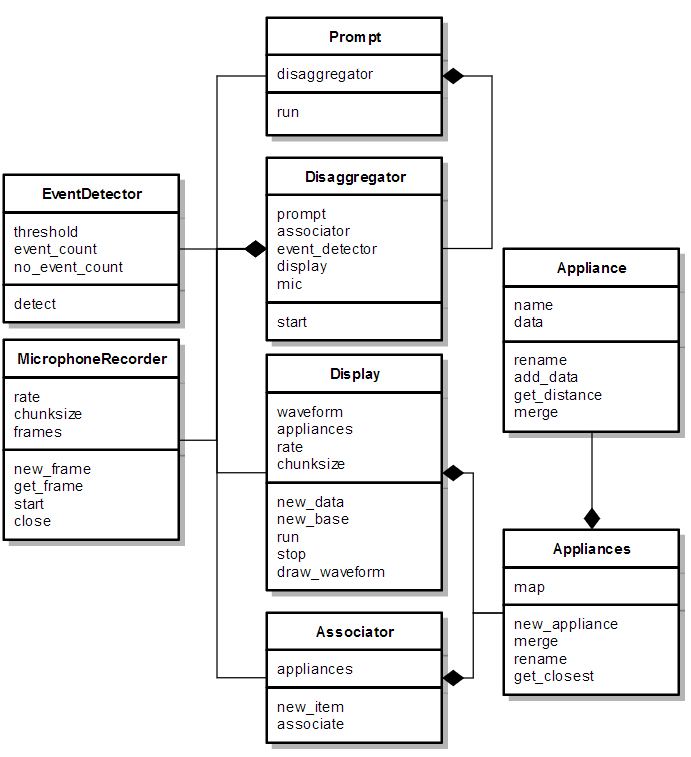
\includegraphics[width=\textwidth]{img/diagram.png}
    \caption{Class Diagram}
    \label{fig:class_diagram}
\end{figure}

\section{Algorithms chosen}
\subsection{KNN}
\subsubsection{Why?}

\subsubsection{}
curse dimentionnality
tree
clustering -> thread
distance -> normalization ?
\section{Tools}